\documentclass{article}
\usepackage[paperwidth=20cm,paperheight=34cm,margin=0.5cm]{geometry}
\usepackage{tikz}
\usepackage{xcolor}
\pagestyle{empty}
\usetikzlibrary{shapes.geometric, arrows.meta, positioning, fit, backgrounds, shadows}

% --- Colour palette ---
\definecolor{stageblue}{HTML}{1A3C5E}
\definecolor{stagecyan}{HTML}{2196F3}
\definecolor{stagegreen}{HTML}{2E7D32}
\definecolor{stageorange}{HTML}{E65100}
\definecolor{stagepurple}{HTML}{4A148C}
\definecolor{stagegray}{HTML}{455A64}
\definecolor{arrowcol}{HTML}{37474F}
\definecolor{boxbg}{HTML}{F5F9FF}
\definecolor{panelbg}{HTML}{ECEFF1}

% --- TikZ styles ---
\tikzset{
  stage/.style={
    rectangle, rounded corners=6pt,
    draw=#1!80!black, fill=#1!15,
    text width=3.4cm, align=center,
    minimum height=1.0cm, font=\small\bfseries,
    drop shadow
  },
  artifact/.style={
    rectangle, rounded corners=4pt,
    draw=stagegray!70, fill=white,
    text width=4.2cm, align=center,
    minimum height=0.85cm, font=\small,
    drop shadow
  },
  phasebox/.style={
    rectangle, rounded corners=4pt,
    draw=stagegreen!60, fill=stagegreen!8,
    text width=7cm, align=left,
    minimum height=0.75cm, font=\footnotesize,
    inner sep=6pt
  },
  evalbox/.style={
    rectangle, rounded corners=4pt,
    draw=stagepurple!60, fill=stagepurple!8,
    text width=4cm, align=center,
    minimum height=0.85cm, font=\footnotesize,
    drop shadow
  },
  sectionlabel/.style={
    font=\small\bfseries\sffamily, text=#1
  },
  arr/.style={-{Stealth[length=7pt]}, thick, color=arrowcol},
}

\begin{document}
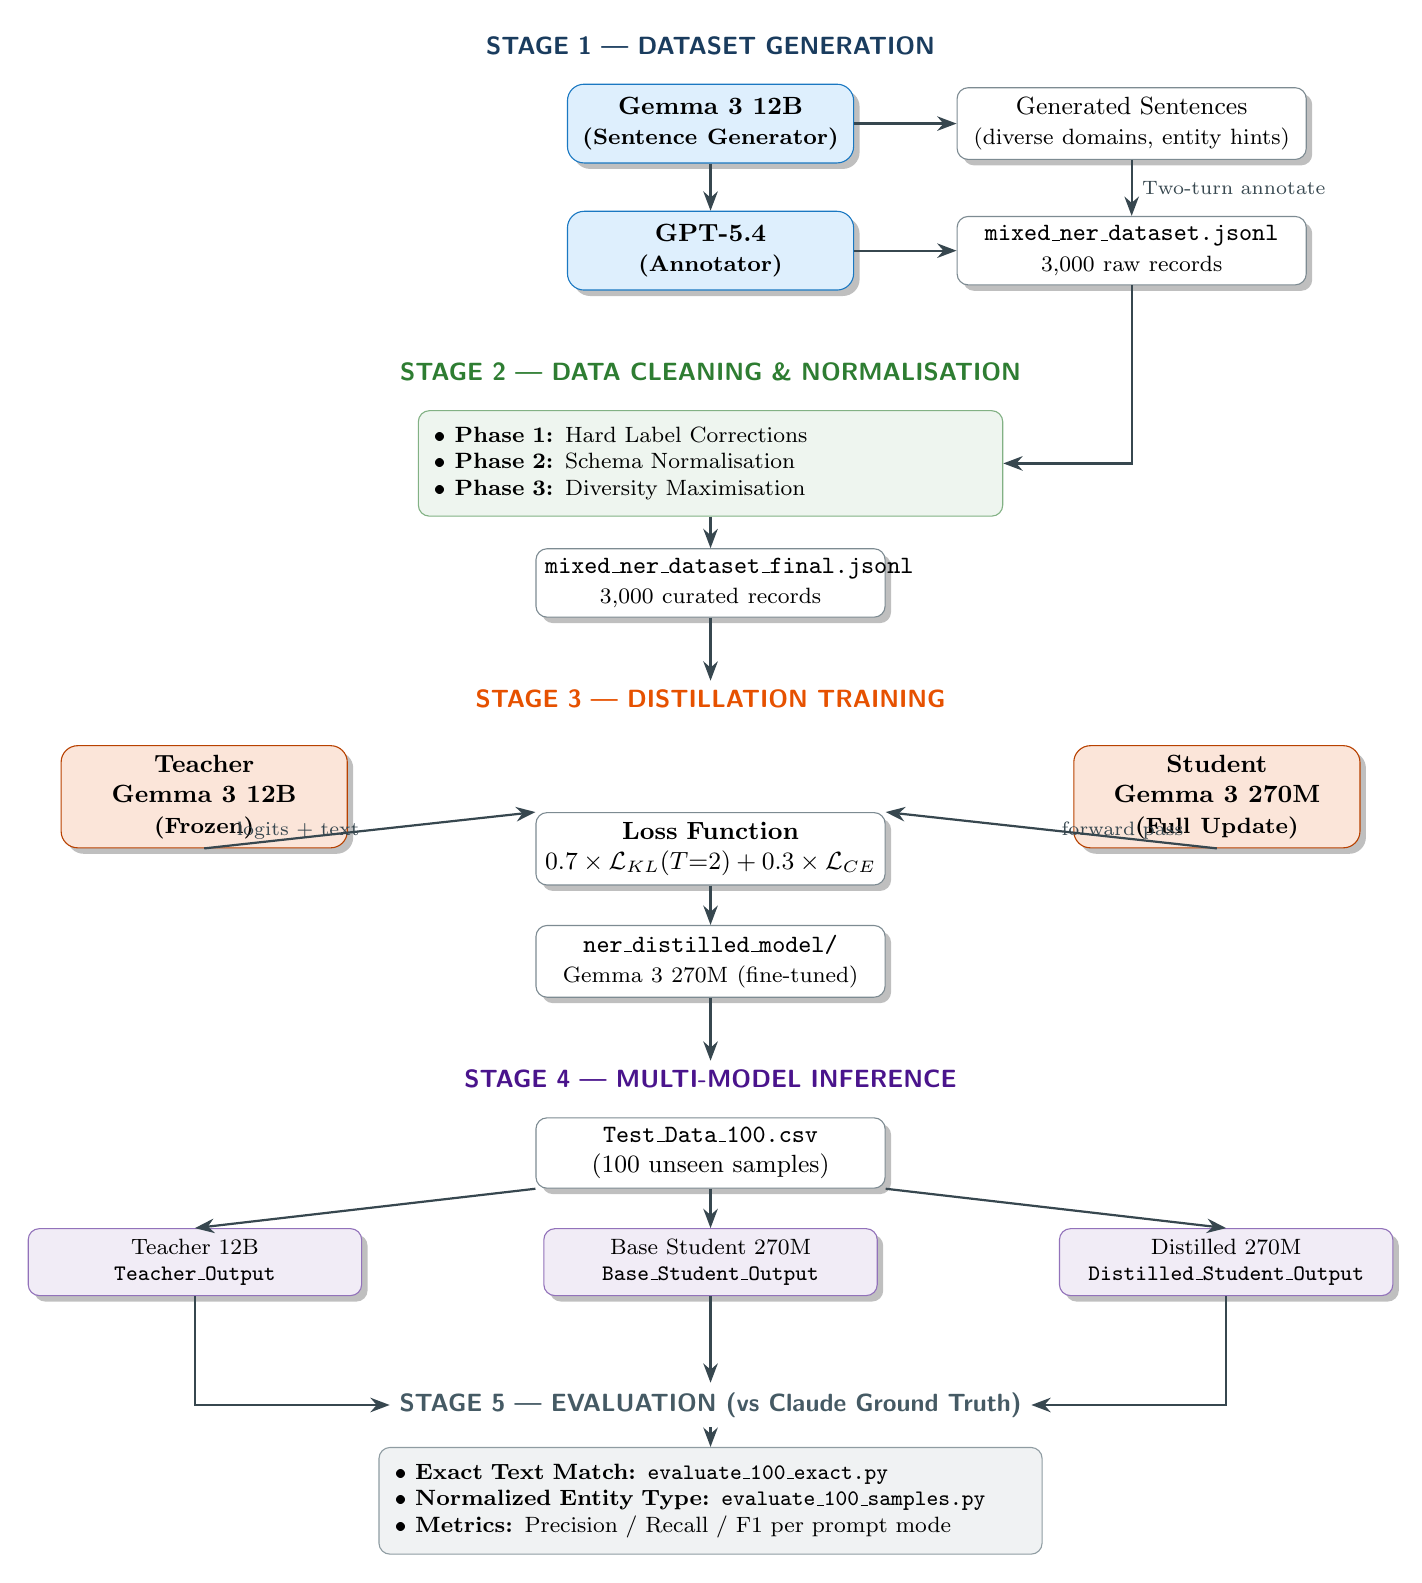
\begin{tikzpicture}[node distance=0.6cm and 1.2cm]

%% ─── STAGE 1: DATASET GENERATION ───
\node[sectionlabel=stageblue] (s1label) {\textsf{STAGE 1 — DATASET GENERATION}};

\node[stage=stagecyan, below=0.25cm of s1label] (gemma12b)
  {Gemma 3 12B\\{\footnotesize(Sentence Generator)}};

\node[artifact, right=1.3cm of gemma12b] (sentences)
  {Generated Sentences\\{\footnotesize(diverse domains, entity hints)}};

\node[stage=stagecyan, below=0.6cm of gemma12b] (gpt54)
  {GPT-5.4\\{\footnotesize(Annotator)}};

\node[artifact, right=1.3cm of gpt54] (rawds)
  {\texttt{mixed\_ner\_dataset.jsonl}\\{\footnotesize 3,000 raw records}};

\draw[arr] (gemma12b) -- (sentences);
\draw[arr] (sentences) -- node[right, font=\scriptsize]{Two-turn annotate} (rawds);
\draw[arr] (gpt54.east) -- (rawds.west);
\draw[arr] (gemma12b) -- (gpt54);

%% ─── STAGE 2: CLEANING ───
\node[sectionlabel=stagegreen, below=0.8cm of gpt54] (s2label)
  {\textsf{STAGE 2 — DATA CLEANING \& NORMALISATION}};

\node[phasebox, below=0.25cm of s2label] (phase1)
  {\textbullet~\textbf{Phase 1:} Hard Label Corrections\\
   \textbullet~\textbf{Phase 2:} Schema Normalisation\\
   \textbullet~\textbf{Phase 3:} Diversity Maximisation};

\node[artifact, below=0.4cm of phase1] (finalds)
  {\texttt{mixed\_ner\_dataset\_final.jsonl}\\{\footnotesize 3,000 curated records}};

\draw[arr] (rawds.south) |- (phase1.east);
\draw[arr] (phase1) -- (finalds);

%% ─── STAGE 3: DISTILLATION TRAINING ───
\node[sectionlabel=stageorange, below=0.8cm of finalds] (s3label)
  {\textsf{STAGE 3 — DISTILLATION TRAINING}};

\node[stage=stageorange, below left=0.35cm and 1.5cm of s3label] (teacher)
  {Teacher\\Gemma 3 12B\\{\footnotesize(Frozen)}};

\node[stage=stageorange, below right=0.35cm and 1.5cm of s3label] (student)
  {Student\\Gemma 3 270M\\{\footnotesize(Full Update)}};

\node[artifact, below=1.2cm of s3label] (loss)
  {\textbf{Loss Function}\\
   $0.7 \times \mathcal{L}_{\text{KL}}(T{=}2) + 0.3 \times \mathcal{L}_{\text{CE}}$};

\node[artifact, below=0.5cm of loss] (distmodel)
  {\texttt{ner\_distilled\_model/}\\{\footnotesize Gemma 3 270M (fine-tuned)}};

\draw[arr] (finalds) -- (s3label);
\draw[arr] (teacher.south) -- node[left, font=\scriptsize]{logits + text} (loss.north west);
\draw[arr] (student.south) -- node[right, font=\scriptsize]{forward pass} (loss.north east);
\draw[arr] (loss) -- (distmodel);

%% ─── STAGE 4: INFERENCE ───
\node[sectionlabel=stagepurple, below=0.8cm of distmodel] (s4label)
  {\textsf{STAGE 4 — MULTI-MODEL INFERENCE}};

\node[artifact, below=0.25cm of s4label] (testdata)
  {\texttt{Test\_Data\_100.csv} (100 unseen samples)};

\node[evalbox, below left=0.5cm and 2.2cm of testdata] (tout)
  {Teacher 12B\\{\footnotesize\texttt{Teacher\_Output}}};

\node[evalbox, below=0.5cm of testdata] (bsout)
  {Base Student 270M\\{\footnotesize\texttt{Base\_Student\_Output}}};

\node[evalbox, below right=0.5cm and 2.2cm of testdata] (dout)
  {Distilled 270M\\{\footnotesize\texttt{Distilled\_Student\_Output}}};

\draw[arr] (distmodel) -- (s4label);
\draw[arr] (testdata.south west) -- (tout.north);
\draw[arr] (testdata.south) -- (bsout.north);
\draw[arr] (testdata.south east) -- (dout.north);

%% ─── STAGE 5: EVALUATION ───
\node[sectionlabel=stagegray, below=1.1cm of bsout] (s5label)
  {\textsf{STAGE 5 — EVALUATION (vs Claude Ground Truth)}};

\node[phasebox, below=0.25cm of s5label, draw=stagegray!60, fill=stagegray!8, text width=8cm] (evalbox)
  {\textbullet~\textbf{Exact Text Match:} \texttt{evaluate\_100\_exact.py}\\
   \textbullet~\textbf{Normalized Entity Type:} \texttt{evaluate\_100\_samples.py}\\
   \textbullet~\textbf{Metrics:} Precision / Recall / F1 per prompt mode};

\draw[arr] (tout.south) |- (s5label.west);
\draw[arr] (bsout.south) -- (s5label.north);
\draw[arr] (dout.south) |- (s5label.east);
\draw[arr] (s5label) -- (evalbox);

\end{tikzpicture}
\end{document}
